% !TeX spellcheck = de_DE
\documentclass[ngerman]{scrartcl} 
%\KOMAoptions{fontsize=12pt, paper=a4}
%\KOMAoptions{DIV=11}
\usepackage[ngerman]{babel}
\def\nummer{1}
\def\autoren{Cornelius Heiming}
\def\datum{29.04.2025}
\def\titel{Ausbreitung von Signalen auf Leitungen}
%TODO: Name, Nummer, Datum	
\title{Versuch \nummer~-  \titel}
\date{\datum}
\author{Cornelius Heiming}
\usepackage{amsmath, amssymb, amsthm} 
\usepackage{geometry}
\usepackage[utf8]{inputenc}
\usepackage{enumerate}
\usepackage[shortlabels]{enumitem}

\usepackage{../pakete}
\usepackage{../aufgaben}

\pagestyle{fancy}
\fancyhf{}
\rhead{Cornelius Heiming}
\chead{Versuch {\nummer}}
\lhead{\datum}
\rfoot{\thepage}

\addbibresource{../referenzen.bib}
\geometry{a4paper, left=3cm, right=3cm, top=3cm, bottom=3cm}

\newtheorem{theorem}{Satz}
\newtheorem{lemma}[theorem]{Lemma}
\newtheorem{korollar}{Korollar}[section]
\theoremstyle{definition}
\newtheorem{definition}[theorem]{Definition}
\newtheorem{beispiel}[theorem]{Beispiel}
\newtheorem{satz}[theorem]{Satz}

%\displaystyle \lim_{x \to \infty}

\begin{document}
\maketitle
\tableofcontents
\clearpage

% === Einleitung ===
\section{Einleitung}

% === Theorie ====
\section{Theorie}
    \subsection{Halbleiter und Dotierung}
    Halbleiter sind im allgemeinsten Falle Stoffe, die sich unter verschiedenen Umständen wie Leiter oder aber wie Nichtleiter verhalten. Dies liegt an der geringen Anzahl an vorhandenen Ladungsträgern, welche man durch gezielte Verunreinigung des Stoffes (sogennante Dotierung) explizit beeinflussen kann. 

    Konkret verwendet man häufig Kristalle von Elementen mit vier Valenzelektronen (bspw. Silizium oder Germanium), welche mit Elementen der dritten bzw. fünften Hauptgruppe verunreinigt, d.h. dotiert werden. Ersteres liefert einen Mangel an freien Elektronen, um die vervollständigte Kristallstruktur zu erreichen, weshalb diese als p(ositiv)-dotiert gelten. Andersherum sorgen Elemente der fünften Hauptgruppe für einen Elektronenüberschuss, also eine n(egativ)-Dotierung.

    Bringt man nun eine p-Dotierte und eine n-Dotierte Schicht zusammen, können Elektronen übergehen. Dadurch entsteht allerdings eine elektrische Kraft, welches der molekularen Bindungskraft entgegen wirkt, es ergibt sich also ein Gleichgewicht von Kräften. In dem Bereich des Kräftegleichgewichts liegen keine freien Ladungsträger vor, da diese vollständig gebunden sind, d.h. diese Schicht ist nichtleitend. Durch ein äußeres elektrisches Feld (Spannung) kann aber das innere elektrische Feld überlagert werden, was, je nach Richtung der Spannung eine Vergrößerung bzw. Verkleinerung des elektrischen Felds zufolge hat. Ab dem Punkt, an welchem sich äußeres und inneres Feld ausgleichen, liegt keine Grenzschicht mehr vor, die Kombination ist also leitend.  
    \subsection{Diode}
    Eine Diode ist ein elektronisches Bauelement, welches den Strom in genau einer Richtung durchlässt. Man spricht von Durchlass- und Sperrrichtung Diese wird zumeist mit einem Halbleiter, wie oben beschrieben, umgesetzt.
    \begin{figure}[H]
        \centering
        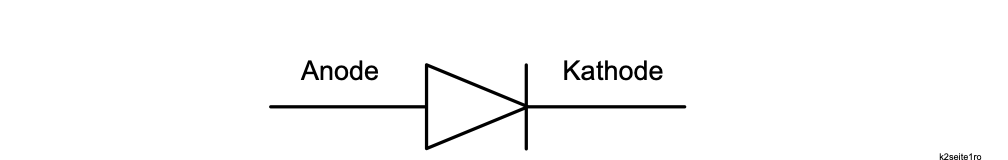
\includegraphics[width=0.8\textwidth]{figs/fig2_1.png}
        \caption{Schaltzeichen Diode}
        \label{fig:Abb2.1}
    \end{figure}

    \subsection{Realität \& Diodenkennlinien}
    In der Realität kann eine Diode die idealisierende Bedingung von Durchlass in einer Richtung und Sperrung in der entgegengesetzten nicht erreichen. In Durchlassrichtung muss zunächst die Grenzschicht mittels eines äußeren Felds überwunden werden, danach verhält sich die Diode wie ein Leiter. In der Sperrichtung kann zunächst stets ein kleiner Strom beobachtet werden, da die freien Ladungsträger der n-dotierten Schicht sich an der Kathode befinden, also einfach abfließen können. Die Elektronen fließen dann durch den Halbleiter nach. Wenn die Spannung in Sperrrichtung groß genug wird, durchbricht die Diode, ist zerstört und leitet den Strom ebenfalls. Dadurch kann man die U-I-Beziehung an einer Diode betrachten - die Diodenkennlinie \ref{fig:Abb2.2}:
    \begin{figure}[H]
        \centering
        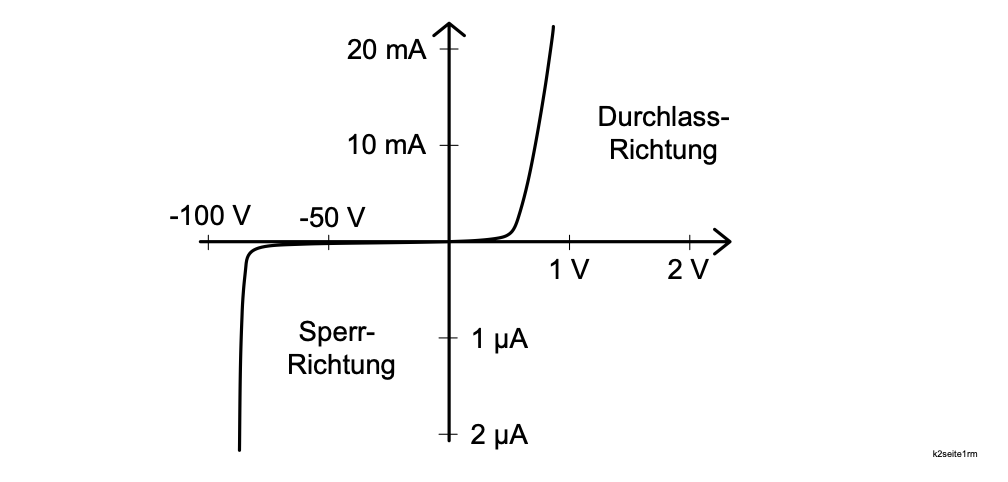
\includegraphics[width=0.8\textwidth]{figs/fig2_2.png}
        \caption{Diodenkennlinie}
        \label{fig:Abb2.2}
    \end{figure}
    \subsection{Gleichrichter}
    Die grundlegende Eigenschaft einer Diode kann verwendet werden, um eine Wechselspannung in eine Gleichspannung umzuwandeln. Am einfachsten geschieht dies durch in-Reihe-Schalten einer Diode, sodass nur Spannungen einer Richtung auftauchen (vgl. \ref{fig:Abb2.4mod} a)). Nachteil daran ist, dass dann mit der Frequenz der Wechselspannnung negative Spannungen, welche durch die Diode annuliert werden, vorliegen. Um dies zu vermeiden, wird ein Zweiweggleichrichter verwendet (vgl. \ref{fig:Abb2.4mod} a)).
    - die Diodenkennlinie \ref{fig:Abb2.2}:
    \begin{figure}[H]
        \centering
        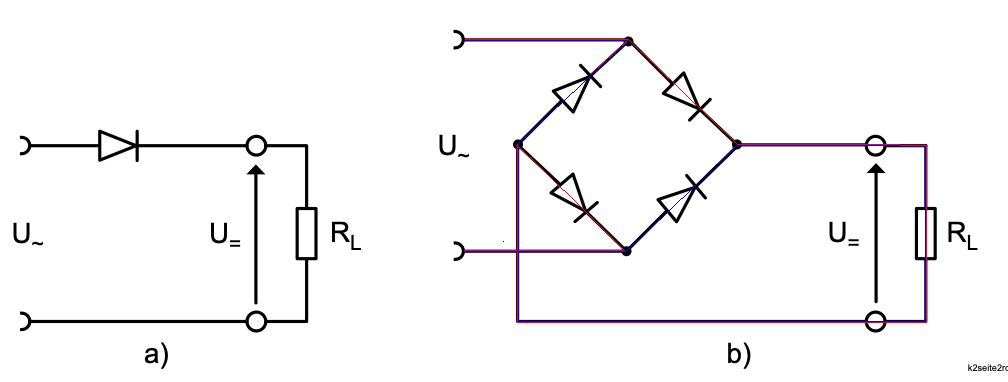
\includegraphics[width=0.8\textwidth]{figs/fig2_4mod.png}
        \caption{Ein- und Zweiweggleichrichter}
        \label{fig:Abb2.4mod}
    \end{figure}
    

    Auch wenn dies die Spannung gleichrichtet, kommen diverse realistische Effekte zu tragen, welche dafür sorgen, dass keine glatte Gleichspannung entsteht, diese Abweichung wird "Brumm" genannt. Um dies nun auch noch auszuglätten wird parallel zum Verbraucher ein Kondensator angelegt.
% === Voraufgaben ===
\section{Voraufgaben}

% == A ==
    \begin{voraufgabe}{Was bestimmt die Dicke der Grenzschicht bei einem p-n-Halbleiter?}
        Die Dicke der Grenzschicht ist abhängig von der Dotierung und dem äußeren elektrischen Feld. Erstere sorgt für die Bereitstellung von Ladungsträgern (Elektronen oder "Löcher"), welche die Grenzschicht bilden und durch das äußere elektrische Feld beeinflusst werden.
    \end{voraufgabe}
% == B ==
    \begin{voraufgabe}{Wie ändert sich die Kapazität einer Diode im Sperrfall mit der angelegten Spannung?}
        Im Sperrfall kann die Diode Modellhaft als Plattenkondensator mit dem Sperrband als Dielektrikum modelliert werden. Für die Dicke des Sperrbands $d$, dessen relative elektische Permeabilität $\epsilon_r$ und die Durchschnittsfläche der Diode $A$ gilt:
        \begin{equation}
            C = \epsilon_0 \epsilon_r \frac{A}{d} \propto \frac{1}{\sqrt{U_\mathrm{ext}}}
            \label{Kapazität einer Diode}
        \end{equation}
    \end{voraufgabe}
    
% == C ==
\begin{voraufgabe}{Skizzieren Sie den Kennlinienverlauf, $I=f(U)$, der Zweipole aus Abb. 2.3 (\ref{fig:Abb2.3}) $(R = \SI{100}{\ohm}; D = \text{Diode})$. Erläutern Sie bei c) und d) den Einfluss der Widerstände.}
    \begin{figure}[H]
        \centering
        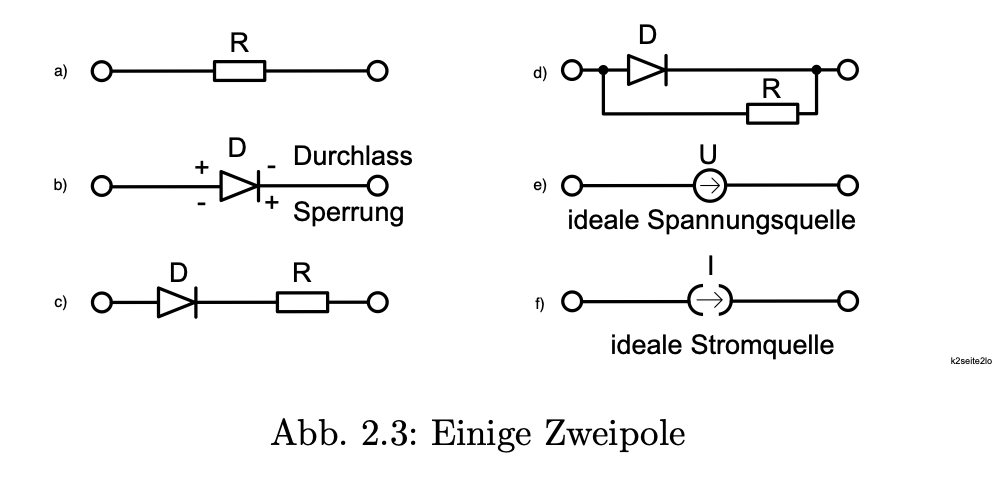
\includegraphics[width=0.8\textwidth]{figs/fig2_3.png}
        \caption{Einige Zweipole}
        \label{fig:Abb2.3}
    \end{figure}
    \begin{figure}[H]
        \centering
        \includegraphics[width=0.8\textwidth, draft]{figs/figC.png}
        \caption{Kennlinienverläufe einiger Zweipole}
        \label{figC}
    \end{figure}

\end{voraufgabe}
% == D ==
\begin{voraufgabe}{Skizzieren Sie den zeitlichen Verlauf der Ausgangsspannungen der Schaltungen in Abb. 2.4 (\ref{fig:Abb2.4}) (a) und (b), wenn die Eingangsspannung eine weit über der Durchlassspannung der Dioden liegende Sinusspannung ist.}
    \begin{figure}[H]
        \centering
        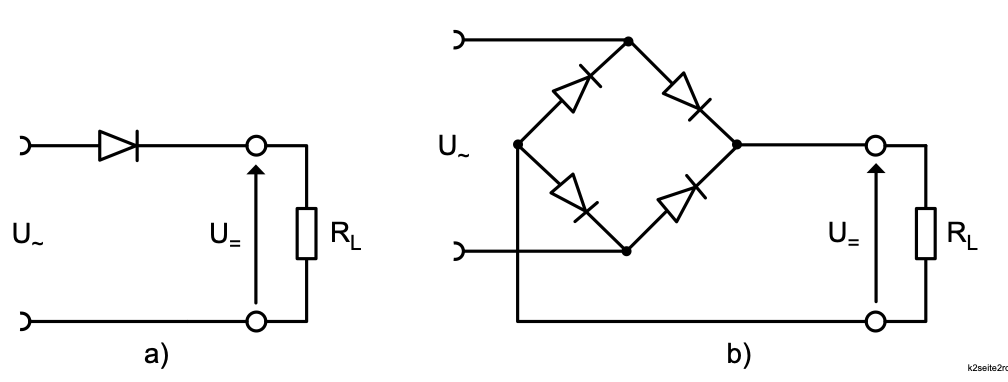
\includegraphics[width=0.8\textwidth]{figs/fig2_4.png}
        \caption{Ein- und Zweiweggleichrichter}
        \label{fig:Abb2.4}
    \end{figure}
    \begin{figure}[H]
        \centering
        \includegraphics[width=0.8\textwidth, draft]{figs/figD.png}
        \caption{Zeitlicher Verlauf der Ausgansspannungen von Ein- und Zweiweggleichrichter}
        \label{figD}
    \end{figure}
\end{voraufgabe}
% == E ==
\begin{voraufgabe}{Wie muss $C$ dimensioniert sein, um die Welligkeit der Spannung über $R$ möglichst klein zu halten?}
Je größer die Kapazität $C$, desto länger dauert der Entladevorgang des Kondensators, was eine längere Kompensation des Brummens und somit eine stärkere Stabilisierung der Ausgansspannung zufolge hat.

\end{voraufgabe}
% == F ==
\begin{voraufgabe}{Wie würden Sie Strom- und Spannungsmessgerät zur Messung der Kennlinie in Durchlassrichtung und in Sperrrichtung anordnen? Berückstichtigen Sie die Innenwiderstände der beiden Geräte.}
Im Allgemeinen müssen Strommessgeräte in Reihe und Spannungsmessgeräte parallelgeschaltet werden. In Sperrichtung hat die Diode einen vergleichsweise hohen Widerstand, welcher für einen geringen Strom durch die Diode sorgt. Dieser sollte möglichst genau gemessen werden, weshalb die Spannungsmessung um die Diode und das Strommessgerät herum erfolgen sollte. Andersherum hat die Diode in Durchlassrichtung einen geringen Widerstand, was für einen hohen Strom sorgt, die Abweichung durch eine Spannungsmessung direkt an der Diode sind also eher gering, also zu bevorzugen.

\end{voraufgabe}
% == G ==
\begin{voraufgabe}{Wie kann man sich eine zu einem Strom proportionale Spannung herstellen?}
    Über einen ohmschen Widerstand fällt die Spannung proportional zur Stromstärke ab.
    \begin{figure}[H]
        \centering
        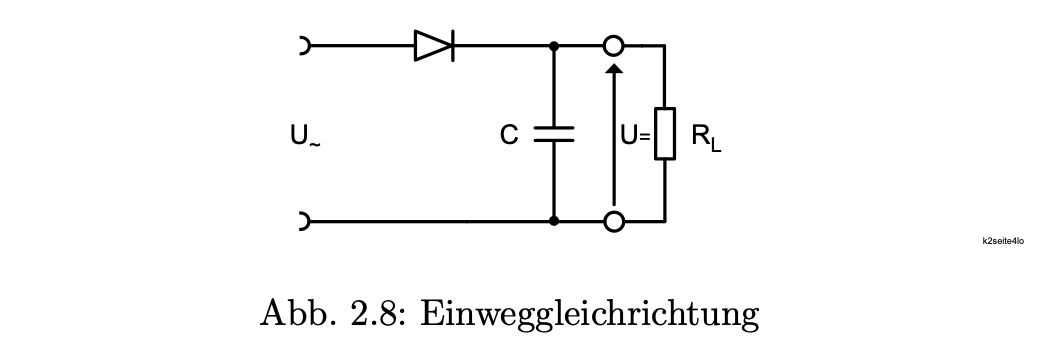
\includegraphics[width=0.8\textwidth]{figs/fig2_8.png}
        \caption{Einweggleichrichtung}
        \label{fig:Abb2.8}
    \end{figure}

\end{voraufgabe}
% == H ==
\begin{voraufgabe}{Für Abb. 2.8 (\ref{fig:Abb2.8}): Berechnen Sie größenordnungsmäßig die größte Kapazität, die benutzt werden darf, ohne die Grenzwerte der Si-Diode zu überschreiten. Nehmen Sie dazu an, dass sich $U$ beim Einschalten um $\SI{1}{\volt}$ in $\SI{100}{\micro\second}$ ändert und vernachlässigen Sie den Einfluss von $R_L$.}
Der Maximalstrom $I_\mathrm{max}$ einer Si-Diode beträgt $\SI{1000}{\milli\ampere}$ (Seite 27 der Anleitung\cite{anleitung}). Wegen Ladungserhaltung gilt:
\begin{equation*}
    C_\mathrm{max} \Delta U = I_\mathrm{max} \Delta t
\end{equation*}
Also:
\begin{equation*}
    C_\mathrm{max} = I_\mathrm{max} \frac{\Delta t}{\Delta U} = \SI{1}{\ampere} \frac{\SI{100}{\micro\second}}{\SI{1}{\volt}} = \SI{100}{\micro\farad}
\end{equation*}
\end{voraufgabe}
% == I ==
\begin{voraufgabe}{Skizzieren Sie den zeitlichen Verlauf der Spannung am Ausgang der Schaltungen in Abb. 2.9.}
    \begin{figure}[H]
        \centering
        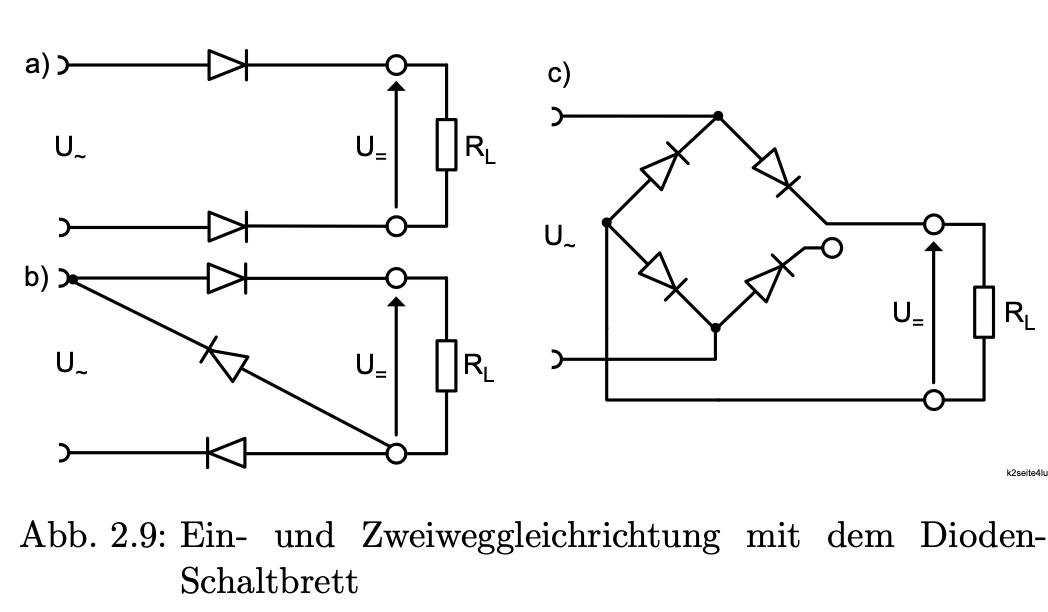
\includegraphics[width=0.8\textwidth]{figs/fig2_9.png}
        \caption{Ein- und Zweiweggleichrichtung mit dem Diodenschaltbrett}
        \label{fig:Abb2.9}
    \end{figure}
    \begin{figure}[H]
        \centering
        \includegraphics[width=0.8\textwidth, draft]{figs/figI.png}
        \caption{Zeitlicher Verlauf der Spannung am Ausgang der Ein- und Zweiweggleichrichtungsschaltungen}
        \label{figI}
    \end{figure}
\end{voraufgabe}
% == J ==
\begin{voraufgabe}{Skizzieren Sie die Lastabhängigkeit der Spannung $U'$ der Schaltung auf der linken Seite in Abb. 2.11. Geben Sie die Formel an, aus der sich $U'$ in Abhängigkeit von $U_0$,$R$ und $R_L$ berechnen lässt. Was sind die Extremwerte für $U'$ und $I$?}
    \begin{figure}[H]
        \centering
        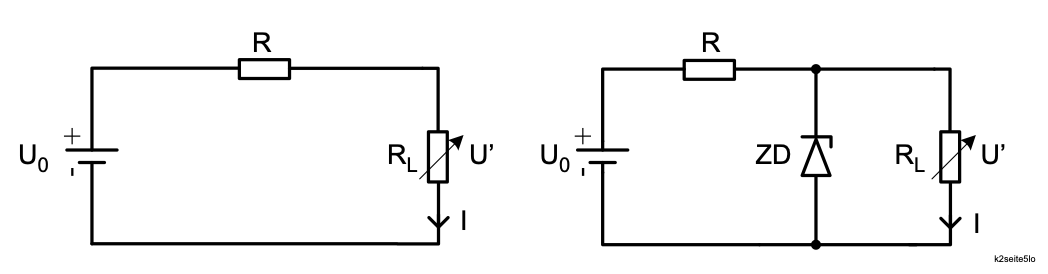
\includegraphics[width=0.8\textwidth]{figs/fig2_11.png}
        \caption{Spannungsstabilisierung mittels Zenerdiode}
        \label{fig:Abb2.11}
    \end{figure}
    \begin{figure}[H]
        \centering
        \includegraphics[width=0.8\textwidth, draft]{figs/figJ.png}
        \caption{Lastabhängigkeit der Spannung $U'$}
        \label{figJ}
    \end{figure}
    Gemäß Kirchhoff gilt:
    \begin{align*}
        U_0 &= R I + R_L I\\
        U' &= I R_L
        \implies U' = U_0 \frac{R_L}{R+R_L}
    \end{align*}
    Da $R$ und $R_L$ nichtnegativ sind, gilt:
    \begin{align*}
        U_\mathrm{\max{}}' &= U_0 \\
        U_\mathrm{\min{}}' &= 0 \\
        I_\mathrm{\max{}}' &= \frac{U_0}{R} \\
        I_\mathrm{\min{}}' &= 0
    \end{align*}

\end{voraufgabe}
% == K ==
\begin{voraufgabe}{Innerhalb welches \underline{Wertebereiches} muss bei dieser Dimensionierung der Arbeitswiderstand $R$ liegen, damit die Ausgangsspannung $U'$ bei der Zenerspannung von $\SI{8.2}{\volt}$ stabilisiert wird?}
    Betriebsdaten der Zenerdiode:
    \begin{align*}
        U_\mathrm{Z}&=\SI{8.2}{\volt}\\
        U_\mathrm{0,max}&=\SI{22}{\volt}\\
        U_\mathrm{0,min}&=\SI{16}{\volt}\\
        I_\mathrm{Z,max}&=\SI{100}{\milli\ampere}\\
        I_\mathrm{Z,min}&=\SI{2}{\milli\ampere}
    \end{align*}
    Falls $R_\mathrm{L}=\infty$, läuft der gesamte Strom durch die Zenerdiode. Dieser darf $I_\mathrm{Z,max}$ nicht überschreiten. Daher muss $R_\mathrm{min}$ entsprechend gewählt werden:
    \begin{align*}
        I_\mathrm{R}&=I_\mathrm{Z,max}=\frac{U_\mathrm{0,max}-U_\mathrm{Z}}{R}\\
        \Rightarrow R&>\frac{U_\mathrm{0,max}-U_\mathrm{Z}}{I_\mathrm{Z,max}}=\SI{138}{\ohm}
    \end{align*}
    Weiterhin darf unter keinen Umständen der Wert für $I_\mathrm{Z,min}=\SI{2}{\milli\ampere}$ unterschritten werden. Hierfür muss der Fall $U_0=U_\mathrm{0,min}$ und $R_\mathrm{L}=\SI{200}{\ohm}$ betrachtet werden:
    \begin{align*}
        I_\mathrm{Z,min} &= I_\mathrm{R}-I_\mathrm{L} \\
        &= \frac{U_\mathrm{0,min}-U_\mathrm{Z}}{R}-\frac{U_\mathrm{Z}}{R_\mathrm{L,min}} \\
        \Rightarrow R &< \frac{U_\mathrm{0,min}-U_\mathrm{Z}}{I_\mathrm{Z,min}+\frac{U_\mathrm{Z}}{R_\mathrm{L,min}}} = \SI{181}{\ohm}
    \end{align*}    
\end{voraufgabe}



% === Aufbau, Durchführung, Messwerte und Auswertung ===
\section{Versuchsaufbau, -durchführung, Messwerte und Auswertung}


% === Fazit ===
\section{Fazit}


\end{document}